\documentclass[12pt]{amsbook}
\usepackage{geometry}                % See geometry.pdf to learn the layout options. There are lots.
%\geometry{letterpaper}                   % ... or a4paper or a5paper or ... 
\geometry{a4paper, top=25mm, right=25mm, bottom=25mm}
%\geometry{landscape}                % Activate for rotated page geometry
\usepackage[parfill]{parskip}    % Activate to begin paragraphs with an empty line rather than an indent
\usepackage{relsize}             % Allows us to define \bigast
\usepackage{graphicx}
\usepackage{amssymb}
\usepackage{epstopdf}
%\usepackage{pause}
\usepackage{wasysym}            % Provides \checkmark
\usepackage[firstpage]{draft watermark}             % Allows the watermark stuff
\usepackage{wrapfig}
\DeclareGraphicsRule{.tif}{png}{.png}{`convert #1 `dirname #1`/`basename #1 .tif`.png}

\newcommand{\DD}{\displaystyle}

\begin{document}
\pagenumbering{gobble}       % This kills the page numbering

\SetWatermarkText{
\begin{minipage}[c][8cm]{8cm}
\begin{center}
 
\end{center}
\end{minipage}
}
\SetWatermarkScale{1.5}
\SetWatermarkColor[gray]{0.75}



\begin{center}
   \textsc{\large MATH 255, Spring 2019 Syllabus}
\end{center}
\vspace{.5cm}

\textbf{Course Title:} Calculus for Biological Scientists II

\textbf{Time/Location:} MTWF, 12:00-12:50 pm, Engineering E205. 

\textbf{Office Hours:} T 1-2PM, W 5-6PM, R 12-1PM

\textbf{Instructor:} Colin Roberts, robertsp@rams.colostate.edu

\textbf{Textbook:} \emph{The Chemistry Maths Book} - $2^{\text{nd}}$ Edition, Erich Steiner

\textbf{Calculator:} Will not be allowed on exams.  Don't worry, the problems given won't make one necessary.

\textbf{Content:} From the course catalog: ``[d]erivatives and integrals of functions of several variables, differential and difference equations, matrices, [and] applications in the biosciences." The semester will be split into three main parts.
\begin{itemize}
\item[] Part 1 - Linear Algebra, Chapters 16, 17, 18, 19
\item[] Part 2 - Multivariate Calculus, Chapters 8, 9, 10
\item[] Part 3 - Differential Equations, Chapters 11, 12, 14
\end{itemize}

\textbf{Grading:} Letter grades will correspond to 10\% windows: 90-100\% is an A, 80-89\% is a B, etc. The following items will contribute to your final grade.
\begin{itemize}
\item[] Exams (50\%) - There will be three exams, one for each of the three parts above. These will happen in class, at dates specified several weeks in advance.
\item[] Project (20\%) - In lieu of a final, we will do a project presentation (potentially in groups). More details about this will be forthcoming.
\item[] Homework (30\%) - Assignments will be given most weeks, usually using questions taken from the textbook. Solutions will be graded on correctness and clarity of supporting work. For example, complete sentences are expected.
\end{itemize}



\begin{wrapfigure}{r}{0.25\textwidth}
%\centering\hspace{.5cm}
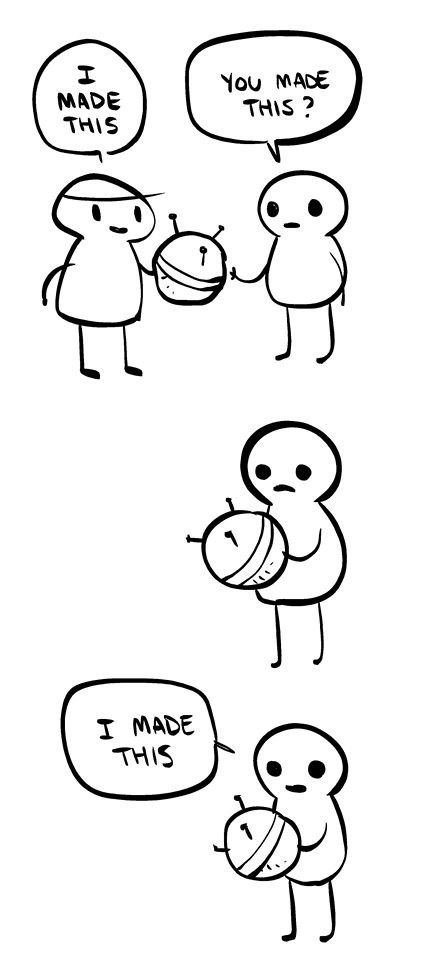
\includegraphics[width=0.25\textwidth]{imadethiscomic.jpg}
\end{wrapfigure}

\textbf{Academic Integrity:} Don't cheat. Check out \texttt{http://tilt.colostate.edu/integrity} for more details. While many things in life operate on the ``better to ask forgiveness than permission" principle, this is not one of them. When in doubt, ask me ahead of time.

Groupwork, unless specified otherwise, is \emph{not} considered cheating in this class, and is very strongly \emph{encouraged}. However, you are expected to write up your solutions individually; word-for-word reproductions look fishy at best, so please make sure to write things in your own words.

\textbf{RDS:} Have a Resources for Disabled Students (RDS) situation? No problem; just let me know as soon as possible.

\textbf{Late Homework:} In general, no late work will be accepted. You'll be asked to turn in homework at the beginning of class on whichever day it is due, though you can always turn it in early. Exceptions for extreme circumstances and emergencies, accompanied by written documentation of proof, will be considered but not guaranteed.

\textbf{Exam Conflicts:} If you are going to miss an exam for a university-sponsored event, provide the appropriate documentation at least a week ahead of time. Encourage your grandparents to stay healthy, as exam-season seems to be an extremely dangerous time for them.

\textbf{Other Expectations:} Treat your classmates and me with respect: silence cell phones when you get to class, don't cause distractions during lecture, don't eat delicious-smelling food without sharing, etc. Homework that is not written legibly or that is a loose collection of papers with no staple will not be accepted (if your handwriting is atrocious, practice or type up your work). Finally, I expect you to give an honest effort and have a good attitude. The number one cause of poor performance in a math class is an ``I can't do it" mentality.

\textbf{Leftovers:} Extra stuff that didn't fit any of the categories above:
\begin{itemize}
\item[] As the instructor, I reserve the right to alter this syllabus at any time. I'll announce any such changes in class, in as timely a manner as possible.
\item[] If you have any issues at all, please do not hesitate to contact me. Pretty much every (non-homework) problem can be resolved via communication.
\item[] Technology is a double-edged sword in learning mathematics. You should attempt to use technology to enhance your understanding without using it as a crutch. Immediately typing the problem into Wolfram Alpha and blindly copying the answer will not help you learn. Plugging the equation for a curve into Desmos (\texttt{https://www.desmos.com/calculator}) to get a good visual before finding a tangent line can be extremely beneficial.
\item[] Related to the above, patience is your biggest ally. You will get stumped from time to time. Resist the urge to immediately ask for help or to right away Google the answer. Instead, try different things; see what you can do with the tools given. Draw a picture. Attempt to do the stupidest, most straight-forward thing possible, and work from there. The process of exploring questions and actively struggling with them will be the most helpful aspect of the class. Don't be Flanders Sr.:
\end{itemize}
\begin{center}
\includegraphics[scale=.65]{triednothing.jpg}\end{center}

\end{document}  